\section{Onboard Debug LEDs}
\label{group__ro__leds}\index{Onboard Debug LEDs@{Onboard Debug LEDs}}
Routines for controlling the onboard Debug LEDs.  
\subsection*{Functions}
\begin{CompactItemize}
\item 
int {\bf set\_\-led} (char led)
\item 
int {\bf clear\_\-led} (char led)
\item 
int {\bf toggle\_\-led} (char led)
\item 
void {\bf led\_\-pwm\_\-fade} (void)
\end{CompactItemize}


\subsection{Detailed Description}
Routines for controlling the onboard Debug LEDs. 



\begin{Code}\begin{verbatim} #include <leds.h> 
\end{verbatim}\end{Code}



This Routines are for setting, clearing and toggeling the four onboard LEDs

\begin{Desc}
\item[Note:]Based on Atmel Datasheet for Atmega128, Nov. 2006 \end{Desc}
\begin{Desc}
\item[Author:]Rainer Ostendorf \end{Desc}


\subsection{Function Documentation}
\index{ro_leds@{ro\_\-leds}!clear_led@{clear\_\-led}}
\index{clear_led@{clear\_\-led}!ro_leds@{ro\_\-leds}}
\subsubsection{\setlength{\rightskip}{0pt plus 5cm}int clear\_\-led (char {\em led})}\label{group__ro__leds_ga07cffc8acf23fbbc1dab7a3d86f7fc7}


turn off the given led \begin{Desc}
\item[Parameters:]
\begin{description}
\item[{\em led}]number of the led to turn off (0-3) \end{description}
\end{Desc}
\begin{Desc}
\item[Returns:]-1 if led has illegal value, 0 else \end{Desc}


Definition at line 57 of file leds.c.\index{ro_leds@{ro\_\-leds}!led_pwm_fade@{led\_\-pwm\_\-fade}}
\index{led_pwm_fade@{led\_\-pwm\_\-fade}!ro_leds@{ro\_\-leds}}
\subsubsection{\setlength{\rightskip}{0pt plus 5cm}void led\_\-pwm\_\-fade (void)}\label{group__ro__leds_g06fabe845524f7bb5beec36a96e7a1bf}


led the leds 1 and 3 fade in and out. BEWARE: this functions uses busy waiting and wastes a huge amount of cpu-time! 

Definition at line 84 of file leds.c.

References delay\_\-ms(), and toggle\_\-led().

Here is the call graph for this function:\begin{figure}[H]
\begin{center}
\leavevmode
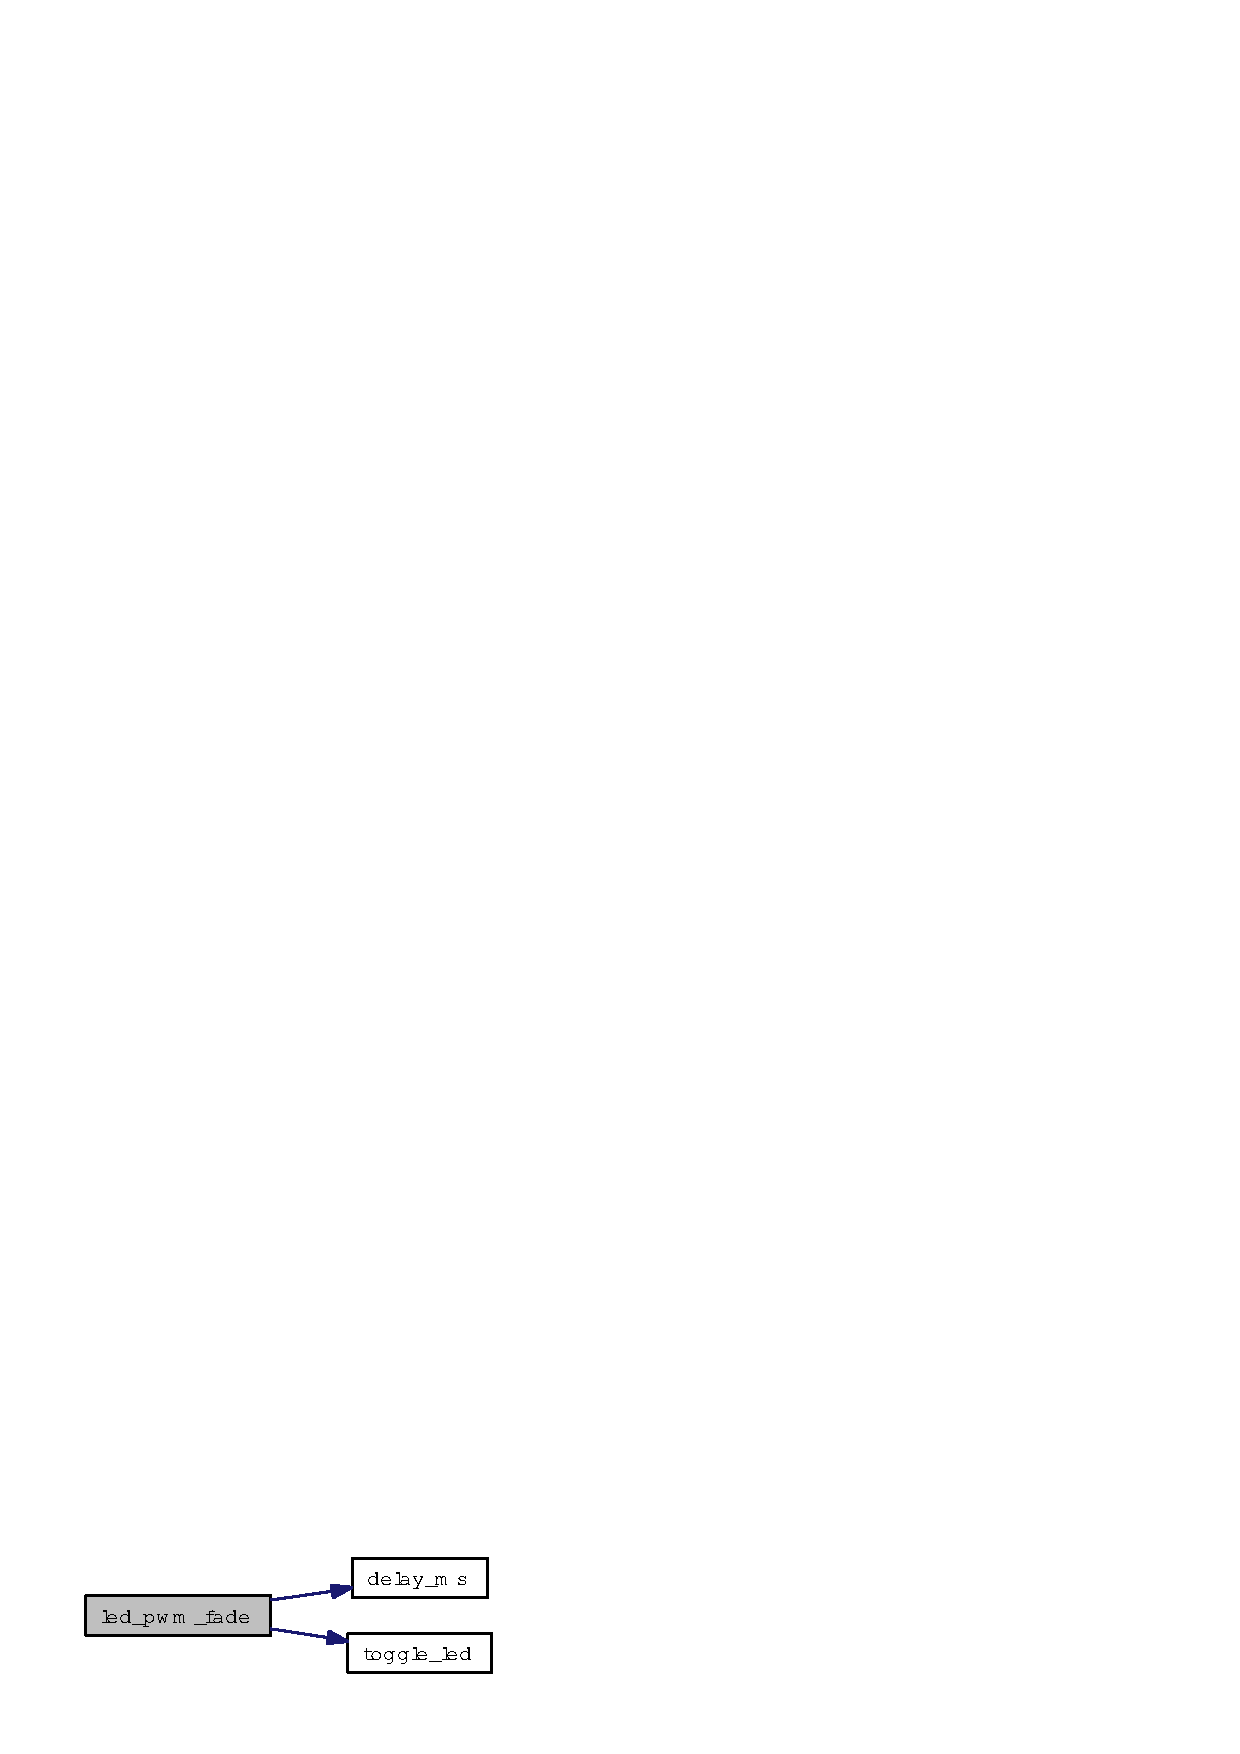
\includegraphics[width=120pt]{group__ro__leds_g06fabe845524f7bb5beec36a96e7a1bf_cgraph}
\end{center}
\end{figure}
\index{ro_leds@{ro\_\-leds}!set_led@{set\_\-led}}
\index{set_led@{set\_\-led}!ro_leds@{ro\_\-leds}}
\subsubsection{\setlength{\rightskip}{0pt plus 5cm}int set\_\-led (char {\em led})}\label{group__ro__leds_gf43daf62ed84fb33cddaf60747a82632}


turn on the given led \begin{Desc}
\item[Parameters:]
\begin{description}
\item[{\em led}]number of the led to turn on (0-3) \end{description}
\end{Desc}
\begin{Desc}
\item[Returns:]-1 if led has illegal value, 0 else \end{Desc}


Definition at line 43 of file leds.c.

Referenced by main().\index{ro_leds@{ro\_\-leds}!toggle_led@{toggle\_\-led}}
\index{toggle_led@{toggle\_\-led}!ro_leds@{ro\_\-leds}}
\subsubsection{\setlength{\rightskip}{0pt plus 5cm}int toggle\_\-led (char {\em led})}\label{group__ro__leds_gefd2b64e1afc42f4660a408da854c6d4}


toggle the given led \begin{Desc}
\item[Parameters:]
\begin{description}
\item[{\em led}]number of the led to toggle (0-3) \end{description}
\end{Desc}
\begin{Desc}
\item[Returns:]-1 if led has illegal value, 0 else \end{Desc}


Definition at line 70 of file leds.c.

Referenced by led\_\-pwm\_\-fade().